\documentclass{article}

\usepackage{graphicx}
\usepackage{tikz}
\usepackage{tikzsymbols}
\usetikzlibrary{calc,patterns,shapes.geometric}
\pagestyle{empty}
\usepackage[margin=0pt]{geometry}
\geometry{papersize={14in,12in}}

\def\centerarc[#1](#2)(#3:#4:#5){\draw[#1] ($(#2)+({#5*cos(#3)},{#5*sin(#3)})$) arc (#3:#4:#5);}

\begin{document}
	\begin{figure}
		\centering
		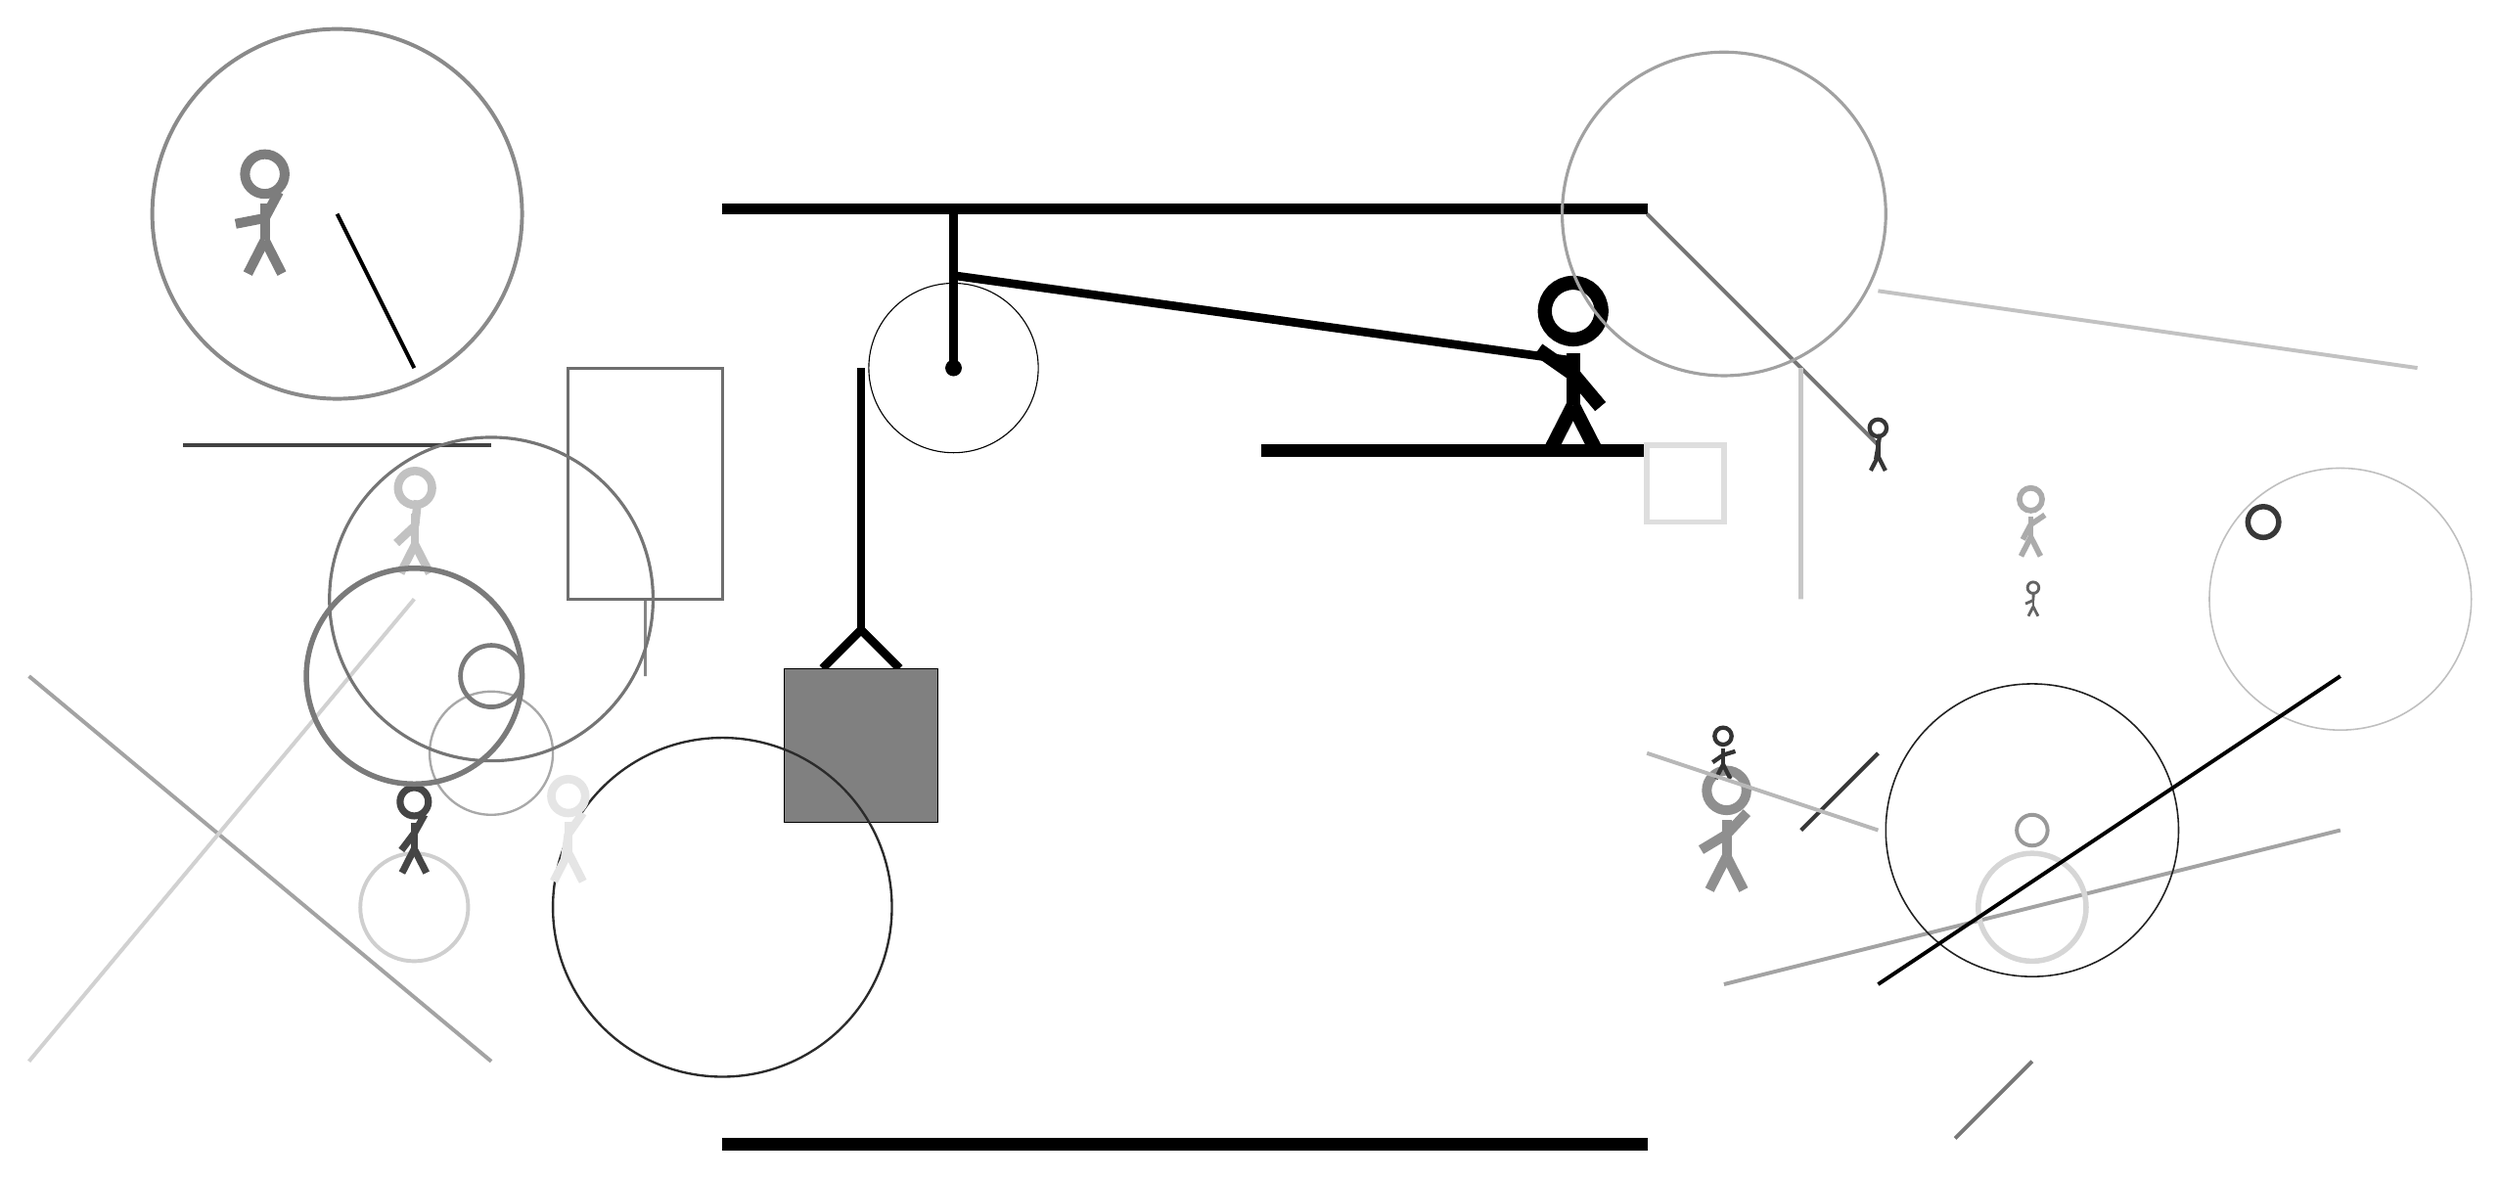
\begin{tikzpicture}
			%%%%% START %%%%%
			
			\draw[fill=black] (-2, 9) rectangle (10, 9.125);
			
			\draw (1, 7) circle (1.1);
			\draw[fill=black] (1, 7) circle (0.1);
			\draw[line width=1.1mm] (1, 9) -- (1, 7);
			
			\draw[line width=1.1mm](-0.7, 3.1) --  (-0.2, 3.6) -- (0.3, 3.1);
			\draw[fill=black!50] (-1.2, 3.1) rectangle (0.8, 1.1);
			
			\draw[line width=1.1mm](-0.2, 7) -- (-0.2, 3.6);
			\centerarc[line width=1.1mm](1, 7)(90:180:1.2000000000000002)
			\draw[line width=1.1mm](1, 8.2) -- (9, 7.1);
			
			\node at (9, 7) {\Strichmaxerl[10][-35][-50]};
			\draw[fill=black] (5, 6) rectangle (10, 5.85);
			
			\draw[line width=0.5mm, color=black!36](11, -1) -- (19, 1);
			
			\draw[line width=0.5mm, color=black!78](13, 2) -- (12, 1);
			\node[line width=0.6mm, color=black!44] at (11, 1) {\Strichmaxerl[7][31][47]};
			\node[line width=0.3mm, color=black!24] at (-6, 5) {\Strichmaxerl[6][43][84]};
			
			\draw[line width=0.5mm, color=black!36](-5, -2) -- (-11, 3);
			\draw[line width=0.5mm, color=black!100](-6, 7) -- (-7, 9);
			\draw [line width=0.2mm, color=black!87](15, 1) circle (1.9);
			\draw [line width=0.3mm, color=black!83](-2, 0) circle (2.2);
			\draw [line width=0.5mm, color=black!19](-6, 0) circle (0.7);
			
			\draw[line width=0.5mm, color=black!54](13, 6) -- (10, 9);
			
			\draw [line width=0.7mm, color=black!16](15, 0) circle (0.7);
			
			\draw[line width=0.5mm, color=black!74](-5, 6) -- (-9, 6);
			\node[line width=0.2mm, color=black!61] at (15, 4) {\Strichmaxerl[2][24][88]};
			\draw [line width=0.2mm, color=black!25](19, 4) circle (1.7);
			\draw[line width=0.4mm, color=black!48] (-3, 3) rectangle (-3, 4);
			\node[line width=0.4mm, color=black!73] at (-6, 1) {\Strichmaxerl[5][53][61]};
			\node[line width=0.6mm, color=black!51] at (-8, 9) {\Strichmaxerl[7][11][62]};
			\draw[line width=0.5mm, color=black!24](13, 8) -- (20, 7);
			\node[line width=0.6mm, color=black!33] at (15, 5) {\Strichmaxerl[4][62][34]};
			
			\draw [line width=0.4mm, color=black!37](11, 9) circle (2.1);
			\draw [line width=0.3mm, color=black!34](-5, 2) circle (0.8);
			
			\draw[line width=0.5mm, color=black!18](-6, 4) -- (-11, -2);
			\node[line width=0.4mm, color=black!80] at (11, 2) {\Strichmaxerl[3][35][17]};
			\draw[line width=0.7mm, color=black!13] (11, 6) rectangle (10, 5);
			\draw[line width=0.5mm, color=black!53](15, -2) -- (14, -3);
			\node[line width=0.2mm, color=black!79] at (13, 6) {\Strichmaxerl[3][80][82]};
			\draw [line width=0.6mm, color=black!52](-5, 3) circle (0.4);
			\draw [line width=0.5mm, color=black!40](15, 1) circle (0.2);
			\draw [line width=0.5mm, color=black!46](-7, 9) circle (2.4);
			
			\draw[line width=0.5mm, color=black!100](13, -1) -- (19, 3);
			\draw[line width=0.6mm, color=black!22] (12, 7) rectangle (12, 4);
			
			\draw[line width=0.4mm, color=black!57] (-2, 4) rectangle (-4, 7);
			\draw [line width=0.4mm, color=black!54](-5, 4) circle (2.1);
			\node[line width=0.7mm, color=black!10] at (-4, 1) {\Strichmaxerl[6][82][55]};
			\draw [line width=0.7mm, color=black!52](-6, 3) circle (1.4);
			\draw[line width=0.5mm, color=black!28](10, 2) -- (13, 1);
			\draw [line width=0.3mm, color=black!89](-7, 2) circle (0.0);
			
			\draw [line width=0.7mm, color=black!78](18, 5) circle (0.2);
			
			\draw[fill=black] (-2, -3) rectangle (10, -3.15);
			
			%%%%% END %%%%%
		\end{tikzpicture}
	\end{figure}	
\end{document}